\documentclass[]{article}
\usepackage{lmodern}
\usepackage{amssymb,amsmath}
\usepackage{ifxetex,ifluatex}
\usepackage{fixltx2e} % provides \textsubscript
\ifnum 0\ifxetex 1\fi\ifluatex 1\fi=0 % if pdftex
  \usepackage[T1]{fontenc}
  \usepackage[utf8]{inputenc}
\else % if luatex or xelatex
  \ifxetex
    \usepackage{mathspec}
  \else
    \usepackage{fontspec}
  \fi
  \defaultfontfeatures{Ligatures=TeX,Scale=MatchLowercase}
\fi
% use upquote if available, for straight quotes in verbatim environments
\IfFileExists{upquote.sty}{\usepackage{upquote}}{}
% use microtype if available
\IfFileExists{microtype.sty}{%
\usepackage{microtype}
\UseMicrotypeSet[protrusion]{basicmath} % disable protrusion for tt fonts
}{}
\usepackage[margin=1in]{geometry}
\usepackage{hyperref}
\hypersetup{unicode=true,
            pdftitle={RMarkdown: Introductory Tutorial},
            pdfauthor={Gabriela Mourão},
            pdfborder={0 0 0},
            breaklinks=true}
\urlstyle{same}  % don't use monospace font for urls
\usepackage{color}
\usepackage{fancyvrb}
\newcommand{\VerbBar}{|}
\newcommand{\VERB}{\Verb[commandchars=\\\{\}]}
\DefineVerbatimEnvironment{Highlighting}{Verbatim}{commandchars=\\\{\}}
% Add ',fontsize=\small' for more characters per line
\usepackage{framed}
\definecolor{shadecolor}{RGB}{248,248,248}
\newenvironment{Shaded}{\begin{snugshade}}{\end{snugshade}}
\newcommand{\KeywordTok}[1]{\textcolor[rgb]{0.13,0.29,0.53}{\textbf{#1}}}
\newcommand{\DataTypeTok}[1]{\textcolor[rgb]{0.13,0.29,0.53}{#1}}
\newcommand{\DecValTok}[1]{\textcolor[rgb]{0.00,0.00,0.81}{#1}}
\newcommand{\BaseNTok}[1]{\textcolor[rgb]{0.00,0.00,0.81}{#1}}
\newcommand{\FloatTok}[1]{\textcolor[rgb]{0.00,0.00,0.81}{#1}}
\newcommand{\ConstantTok}[1]{\textcolor[rgb]{0.00,0.00,0.00}{#1}}
\newcommand{\CharTok}[1]{\textcolor[rgb]{0.31,0.60,0.02}{#1}}
\newcommand{\SpecialCharTok}[1]{\textcolor[rgb]{0.00,0.00,0.00}{#1}}
\newcommand{\StringTok}[1]{\textcolor[rgb]{0.31,0.60,0.02}{#1}}
\newcommand{\VerbatimStringTok}[1]{\textcolor[rgb]{0.31,0.60,0.02}{#1}}
\newcommand{\SpecialStringTok}[1]{\textcolor[rgb]{0.31,0.60,0.02}{#1}}
\newcommand{\ImportTok}[1]{#1}
\newcommand{\CommentTok}[1]{\textcolor[rgb]{0.56,0.35,0.01}{\textit{#1}}}
\newcommand{\DocumentationTok}[1]{\textcolor[rgb]{0.56,0.35,0.01}{\textbf{\textit{#1}}}}
\newcommand{\AnnotationTok}[1]{\textcolor[rgb]{0.56,0.35,0.01}{\textbf{\textit{#1}}}}
\newcommand{\CommentVarTok}[1]{\textcolor[rgb]{0.56,0.35,0.01}{\textbf{\textit{#1}}}}
\newcommand{\OtherTok}[1]{\textcolor[rgb]{0.56,0.35,0.01}{#1}}
\newcommand{\FunctionTok}[1]{\textcolor[rgb]{0.00,0.00,0.00}{#1}}
\newcommand{\VariableTok}[1]{\textcolor[rgb]{0.00,0.00,0.00}{#1}}
\newcommand{\ControlFlowTok}[1]{\textcolor[rgb]{0.13,0.29,0.53}{\textbf{#1}}}
\newcommand{\OperatorTok}[1]{\textcolor[rgb]{0.81,0.36,0.00}{\textbf{#1}}}
\newcommand{\BuiltInTok}[1]{#1}
\newcommand{\ExtensionTok}[1]{#1}
\newcommand{\PreprocessorTok}[1]{\textcolor[rgb]{0.56,0.35,0.01}{\textit{#1}}}
\newcommand{\AttributeTok}[1]{\textcolor[rgb]{0.77,0.63,0.00}{#1}}
\newcommand{\RegionMarkerTok}[1]{#1}
\newcommand{\InformationTok}[1]{\textcolor[rgb]{0.56,0.35,0.01}{\textbf{\textit{#1}}}}
\newcommand{\WarningTok}[1]{\textcolor[rgb]{0.56,0.35,0.01}{\textbf{\textit{#1}}}}
\newcommand{\AlertTok}[1]{\textcolor[rgb]{0.94,0.16,0.16}{#1}}
\newcommand{\ErrorTok}[1]{\textcolor[rgb]{0.64,0.00,0.00}{\textbf{#1}}}
\newcommand{\NormalTok}[1]{#1}
\usepackage{longtable,booktabs}
\usepackage{graphicx,grffile}
\makeatletter
\def\maxwidth{\ifdim\Gin@nat@width>\linewidth\linewidth\else\Gin@nat@width\fi}
\def\maxheight{\ifdim\Gin@nat@height>\textheight\textheight\else\Gin@nat@height\fi}
\makeatother
% Scale images if necessary, so that they will not overflow the page
% margins by default, and it is still possible to overwrite the defaults
% using explicit options in \includegraphics[width, height, ...]{}
\setkeys{Gin}{width=\maxwidth,height=\maxheight,keepaspectratio}
\IfFileExists{parskip.sty}{%
\usepackage{parskip}
}{% else
\setlength{\parindent}{0pt}
\setlength{\parskip}{6pt plus 2pt minus 1pt}
}
\setlength{\emergencystretch}{3em}  % prevent overfull lines
\providecommand{\tightlist}{%
  \setlength{\itemsep}{0pt}\setlength{\parskip}{0pt}}
\setcounter{secnumdepth}{0}
% Redefines (sub)paragraphs to behave more like sections
\ifx\paragraph\undefined\else
\let\oldparagraph\paragraph
\renewcommand{\paragraph}[1]{\oldparagraph{#1}\mbox{}}
\fi
\ifx\subparagraph\undefined\else
\let\oldsubparagraph\subparagraph
\renewcommand{\subparagraph}[1]{\oldsubparagraph{#1}\mbox{}}
\fi

%%% Use protect on footnotes to avoid problems with footnotes in titles
\let\rmarkdownfootnote\footnote%
\def\footnote{\protect\rmarkdownfootnote}

%%% Change title format to be more compact
\usepackage{titling}

% Create subtitle command for use in maketitle
\newcommand{\subtitle}[1]{
  \posttitle{
    \begin{center}\large#1\end{center}
    }
}

\setlength{\droptitle}{-2em}

  \title{RMarkdown: Introductory Tutorial}
    \pretitle{\vspace{\droptitle}\centering\huge}
  \posttitle{\par}
    \author{Gabriela Mourão}
    \preauthor{\centering\large\emph}
  \postauthor{\par}
      \predate{\centering\large\emph}
  \postdate{\par}
    \date{27 de novembro de 2018}


\begin{document}
\maketitle

{
\setcounter{tocdepth}{2}
\tableofcontents
}
 The main goal in this document in cover the very basics formatation for
Rmarkdown, no matter if you are building a Html or pdf document. If you
are new to Rmarkdown, please check the following reference for
instalation guidance:
\url{https://bookdown.org/yihui/rmarkdown/installation.html}

\section{Text Formatation}\label{text-formatation}

\subsection{Basic Formatation}\label{basic-formatation}

\textbf{a. Manual line Break}

To add a line break, you can type two or more spaces in the end of the
line, just like that:\\
\emph{this is a new line}

\textbf{b.Headers type}

\begin{verbatim}
# Header 1
## Header 2
### Header 3
\end{verbatim}

\textbf{c.Text Emphasis}

\emph{- Italic Format}\\
\textbf{- Bold Format}\\
- Subscript\textsubscript{1}\\
- Superscript\textsuperscript{1}

\begin{verbatim}
*Italic* or _italic_
**Bold** or __Bold__
Subscript~1~
Superscript^1^
\end{verbatim}

\subsection{Lists}\label{lists}

\textbf{a. Ordered list}

\begin{verbatim}
1. First Element
2. Second Element
      + Nested Element
      + Another Nested Element
\end{verbatim}

\textbf{b. Unordered list}

\begin{verbatim}
* Text 
* Another text
      + Nested text
- Other option for list
      + Again nested text
\end{verbatim}

\begin{center}\rule{0.5\linewidth}{\linethickness}\end{center}

\subsection{Page Break}\label{page-break}

To add a page break, as the example above, you can simply type four or
more dashes or asteristics:

\begin{verbatim}
------ or 
******
\end{verbatim}

\subsection{Blockquotes}\label{blockquotes}

\textbf{a. Plain Code Block }

Since the beggining of this session I am using this option to show how
to apply each of the formattings introduced up to now. With them it is
possible to write some code in a fixed-width box, but not evaulating it:

\begin{verbatim}
      ```
      This text is displayed as it is **typed!** 
      ```
\end{verbatim}

\textbf{b. Blockquotes}

Can be used to add some quotes in your markdown file, as in the
following example.

\begin{quote}
``No medicine cures what happiness cannot''

\emph{Gabriel Garcia Marques}\\
:)
\end{quote}

\begin{verbatim}
> No medicine cures what happiness cannot  
> *Gabriel Garcia Marques*  
> :)
\end{verbatim}

\begin{center}\rule{0.5\linewidth}{\linethickness}\end{center}

\section{Output formats}\label{output-formats}

There are several outputs formats available in Markdown:

\begin{itemize}
\tightlist
\item
  beamer\_presentation\\
\item
  github\_document\\
\item
  html\_document\\
\item
  ioslides\_presentation\\
\item
  latex\_document\\
\item
  md\_document\\
\item
  odt\_document\\
\item
  pdf\_document\\
\item
  powerpoint\_presentation\\
\item
  rtf\_document\\
\item
  slidy\_presentation\\
\item
  word\_document
\end{itemize}

Up to now, this tutorial have been focusing on markdown syntax in a more
broadly way, But now, lets focus on some options for
\textbf{html\_document} output.\\
If you type ?rmarkdown::html\_document in your R console, you can get a
list of all options for HTML document. The ones that I use most are
described below:

\begin{itemize}
\tightlist
\item
  \textbf{code\_folding:} Enable document readers to toggle the display
  of R code chunks. Specify ``none'' to display all code chunks
  (assuming they were knit with echo = TRUE). Specify ``hide'' to hide
  all R code chunks by default (users can show hidden code chunks either
  individually or document-wide). Specify ``show'' to show all R code
  chunks by default.\\
\item
  \textbf{toc:} to include a table of contents in the output\\
\item
  \textbf{toc\_depth:} Depth of headers to include in table format\\
\item
  \textbf{toc\_float:} TRUE to float the table of contents\\
\item
  \textbf{Code\_download:} Embeded the Rmd source code within the
  document and provide a link that can be used by readers to download
  the code.\\
\item
  \textbf{number\_sections:} TRUE to number section headings
\item
  \textbf{self\_conteained:} Produce a standalone HTML file with no
  external dependencies.
\end{itemize}

\subsection{Usage examples:}\label{usage-examples}

Following you can find some usage examples of the mentioned options:

\begin{verbatim}
      html_document:
            code_folding: show
            toc: yes
            toc_depth: 1
            toc_float: yes
            code_download: yes
            highlight: haddock
            theme: lumen
\end{verbatim}

\begin{figure}
\centering
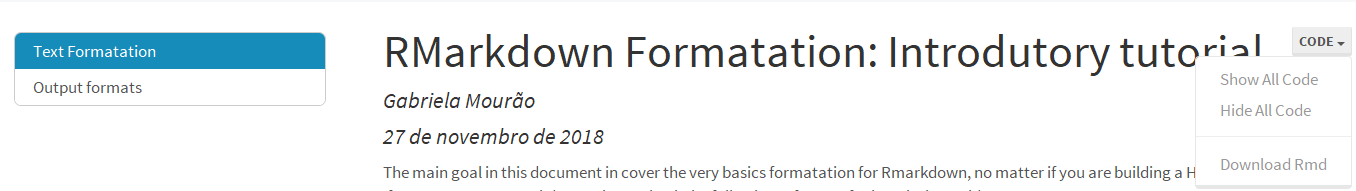
\includegraphics{C:/Users/gabriela.mourao/Documents/6-PESSOAL/R-files/TUTORIAL_MARKDOWN/output1.png}
\caption{}
\end{figure}

\subsection{\texorpdfstring{}{ }}\label{section}

Including section number:

\begin{verbatim}
output: 
      html_document:
            code_folding: show
            toc: yes
            toc_depth: 2
            toc_float: yes
            code_download: yes
            number_sections: true
            highlight: haddock
            theme: lumen
\end{verbatim}

\begin{figure}
\centering
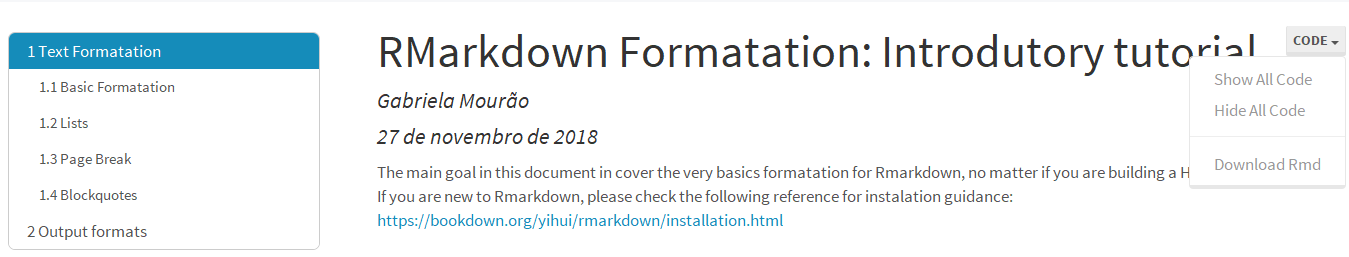
\includegraphics{C:/Users/gabriela.mourao/Documents/6-PESSOAL/R-files/TUTORIAL_MARKDOWN/output2.png}
\caption{}
\end{figure}

\begin{center}\rule{0.5\linewidth}{\linethickness}\end{center}

 Flatly theme:

\begin{figure}
\centering
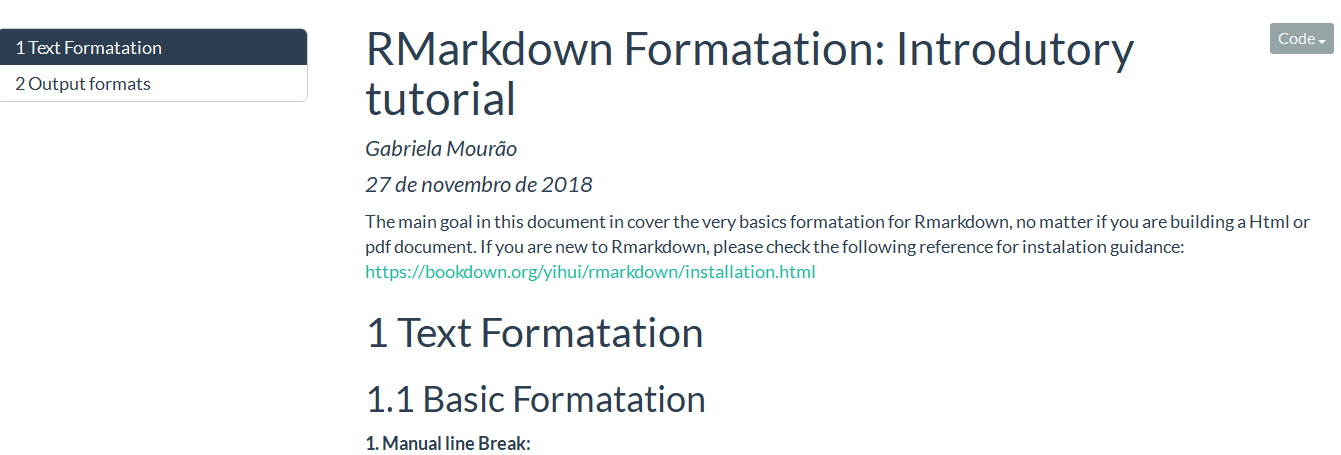
\includegraphics{C:/Users/gabriela.mourao/Documents/6-PESSOAL/R-files/TUTORIAL_MARKDOWN/flatly.png}
\caption{}
\end{figure}

\begin{center}\rule{0.5\linewidth}{\linethickness}\end{center}

Journal theme:\\
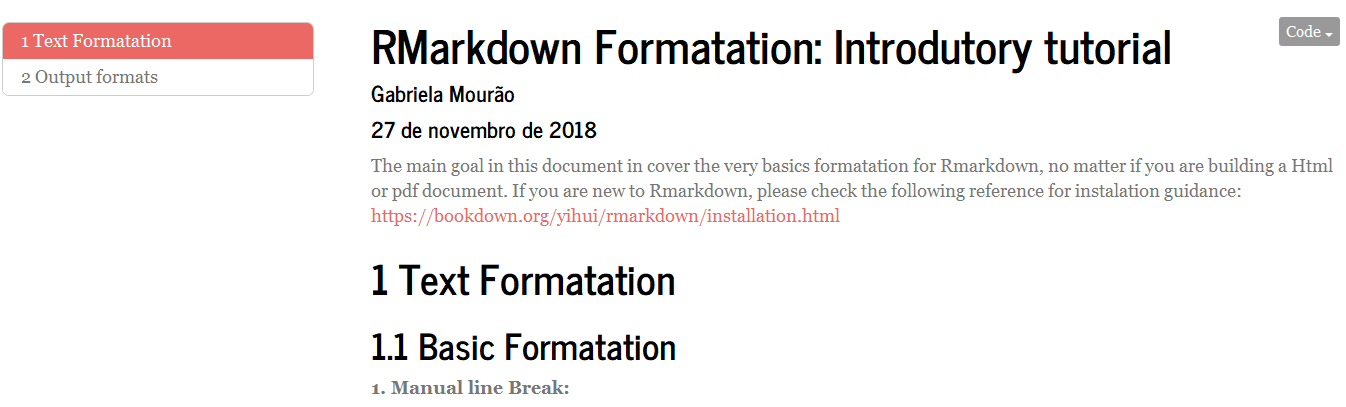
\includegraphics{C:/Users/gabriela.mourao/Documents/6-PESSOAL/R-files/TUTORIAL_MARKDOWN/journal_and_haddock.png}

\begin{center}\rule{0.5\linewidth}{\linethickness}\end{center}

Lumen theme:\\
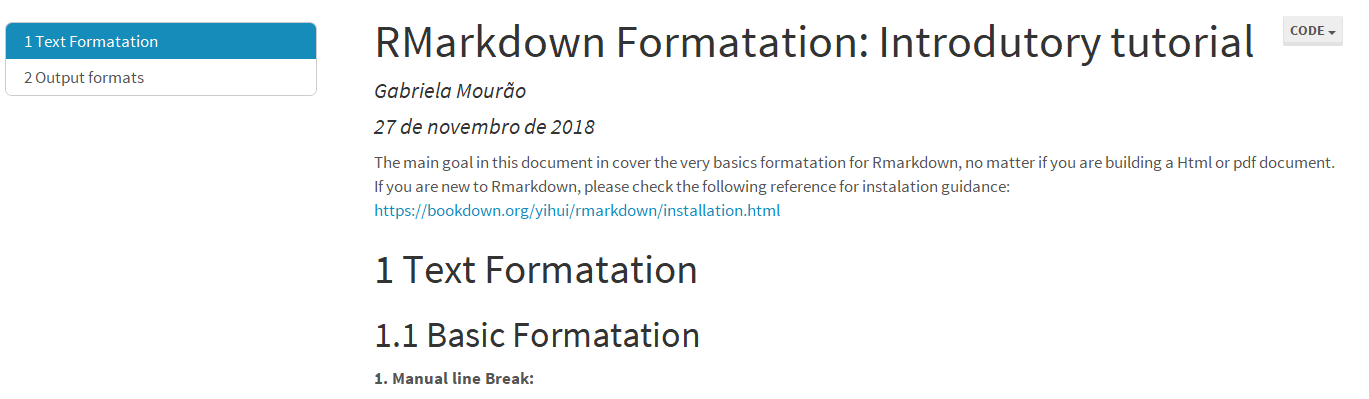
\includegraphics{C:/Users/gabriela.mourao/Documents/6-PESSOAL/R-files/TUTORIAL_MARKDOWN/lumen.png}

\begin{center}\rule{0.5\linewidth}{\linethickness}\end{center}

\section{Code}\label{code}

\subsection{Echo Options}\label{echo-options}

To insert some codes in the markdown document, the called code chunk, it
is necessary to add three backticks like ´´´ followed by \{r\}, where r
indicates the language name. To close the code chunk, add another three
backticks in the end. You can write chunk options in the curly braces,
as we are going to see in the following examples.

\begin{Shaded}
\begin{Highlighting}[]
\KeywordTok{summary}\NormalTok{(cars)}
\end{Highlighting}
\end{Shaded}

\begin{verbatim}
##      speed           dist       
##  Min.   : 4.0   Min.   :  2.00  
##  1st Qu.:12.0   1st Qu.: 26.00  
##  Median :15.0   Median : 36.00  
##  Mean   :15.4   Mean   : 42.98  
##  3rd Qu.:19.0   3rd Qu.: 56.00  
##  Max.   :25.0   Max.   :120.00
\end{verbatim}

Another easier way to add a R code chunk is simply type: ``ctrl + alt +
i''. It is possible to control the code output adding some chunk options
inside the curly braces: \{r \}.\\
Following, some very useful options that I use very frequently:

\begin{itemize}
\tightlist
\item
  \textbf{eval:} TRUE to evaluate the code chunk\\
\item
  \textbf{echo:} TRUE to show the code in the output document\\
\item
  \textbf{results:} If ``hide'' the text output will be hidden, ``asis''
  for write a text as is.\\
\item
  \textbf{collapse:} TRUE to merge output text and the code into a
  single code block in the output.\\
\item
  \textbf{Warning, message and error:} Whether to show warnings,
  messages and error in the output document
\item
  \textbf{include:} When include = FALSE, the whole code chunk is
  excluded in the output, but note that it will still be evaluated if
  eval = TRUE.\\
\item
  \textbf{cache:} If caching is enabled, the same code chunk will not be
  evaluated the next time the document is compiled (if the code chunk
  was not modified), which can save you time.\\
\item
  \textbf{fig.width and fig.height:} The (graphical device) size of R
  plots in inches. Ex: fig.width = 6 and fig.height = 4 or fig.dim =
  c(6, 4).\\
\item
  \textbf{out.width and out.height:} The output size of R plots in the
  output document. These options may scale images. You can use
  percentages, e.g., out.width = `80\%' means 80\% of the page width.\\
\item
  \textbf{fig.align:} The alignment of plots. It can be `left',
  `center', or `right'.\\
\item
  \textbf{fig.cap: } To include some figure caption.
\end{itemize}

For a better understanding of how these options work, we can see some
examples below:

\begin{enumerate}
\def\labelenumi{\arabic{enumi}.}
\tightlist
\item
  \textbf{\{r, include = FALSE\}}

  \begin{itemize}
  \tightlist
  \item
    Code not shown\\
  \item
    results not shown\\
  \end{itemize}
\item
  \textbf{\{r, echo = FALSE\}}

  \begin{itemize}
  \tightlist
  \item
    Code not shown
  \item
    results shown
  \end{itemize}
\end{enumerate}

\begin{verbatim}
##      speed           dist       
##  Min.   : 4.0   Min.   :  2.00  
##  1st Qu.:12.0   1st Qu.: 26.00  
##  Median :15.0   Median : 36.00  
##  Mean   :15.4   Mean   : 42.98  
##  3rd Qu.:19.0   3rd Qu.: 56.00  
##  Max.   :25.0   Max.   :120.00
\end{verbatim}

\begin{enumerate}
\def\labelenumi{\arabic{enumi}.}
\setcounter{enumi}{2}
\tightlist
\item
  \textbf{\{r, results = `hide'\}}

  \begin{itemize}
  \tightlist
  \item
    Code shown\\
  \item
    Results not shown
  \end{itemize}
\end{enumerate}

\begin{Shaded}
\begin{Highlighting}[]
\KeywordTok{summary}\NormalTok{(cars)}
\end{Highlighting}
\end{Shaded}

\begin{enumerate}
\def\labelenumi{\arabic{enumi}.}
\setcounter{enumi}{3}
\tightlist
\item
  \textbf{\{r, collapse=TRUE\}}

  \begin{itemize}
  \tightlist
  \item
    To merge the code and the output
  \end{itemize}
\end{enumerate}

\begin{Shaded}
\begin{Highlighting}[]
\KeywordTok{summary}\NormalTok{(cars)}
\NormalTok{##      speed           dist       }
\NormalTok{##  Min.   : 4.0   Min.   :  2.00  }
\NormalTok{##  1st Qu.:12.0   1st Qu.: 26.00  }
\NormalTok{##  Median :15.0   Median : 36.00  }
\NormalTok{##  Mean   :15.4   Mean   : 42.98  }
\NormalTok{##  3rd Qu.:19.0   3rd Qu.: 56.00  }
\NormalTok{##  Max.   :25.0   Max.   :120.00}
\end{Highlighting}
\end{Shaded}

\begin{enumerate}
\def\labelenumi{\arabic{enumi}.}
\setcounter{enumi}{4}
\tightlist
\item
  \textbf{\{r, out.width=`30\%', fig.align=`center', fig.cap=`Amazing
  Hong Kong'\}}

  \begin{itemize}
  \tightlist
  \item
    Another option for including images and captions.
  \end{itemize}
\end{enumerate}

\begin{Shaded}
\begin{Highlighting}[]
\NormalTok{knitr}\OperatorTok{::}\KeywordTok{include_graphics}\NormalTok{(}\StringTok{'C:/Users/gabriela.mourao/Documents/6-PESSOAL/timon-studler-49992-unsplash.jpg'}\NormalTok{)}
\end{Highlighting}
\end{Shaded}

\begin{figure}

{\centering \includegraphics[width=0.3\linewidth]{C:/Users/gabriela.mourao/Documents/6-PESSOAL/timon-studler-49992-unsplash} 

}

\caption{Amazing Hong Kong}\label{fig:unnamed-chunk-6}
\end{figure}

\begin{enumerate}
\def\labelenumi{\arabic{enumi}.}
\setcounter{enumi}{5}
\tightlist
\item
  \textbf{\{r, fig.align=`center', fig.width = 6, fig.height=4\}}

  \begin{itemize}
  \tightlist
  \item
    It is possible to adjust the graph size as well its alignment in the
    output document
  \end{itemize}
\end{enumerate}

\begin{Shaded}
\begin{Highlighting}[]
\KeywordTok{ggplot}\NormalTok{(cars, }\KeywordTok{aes}\NormalTok{(}\DataTypeTok{x=}\NormalTok{speed, }\DataTypeTok{y=}\NormalTok{dist)) }\OperatorTok{+}
\StringTok{      }\KeywordTok{geom_point}\NormalTok{(}\DataTypeTok{alpha=}\DecValTok{1}\NormalTok{) }\OperatorTok{+}\StringTok{ }
\StringTok{      }\KeywordTok{labs}\NormalTok{(}\DataTypeTok{title =} \StringTok{"Speed vs. Distance"}\NormalTok{, }\DataTypeTok{x =} \StringTok{"Speed"}\NormalTok{, }\DataTypeTok{y =} \StringTok{"Distance"}\NormalTok{) }\OperatorTok{+}\StringTok{ }
\StringTok{      }\KeywordTok{theme_bw}\NormalTok{()}
\end{Highlighting}
\end{Shaded}

\begin{center}\includegraphics{Markdown_formatation_files/figure-latex/unnamed-chunk-7-1} \end{center}

There are many options available for control the Code Chunk output, if
you want more information about it in the following links you can find
good references:\\
\url{https://yihui.name/knitr/options/}\\
\url{https://bookdown.org/yihui/rmarkdown/r-code.html}\\
\url{https://www.overleaf.com/learn/latex/Positioning_images_and_tables}

\subsection{Inline Code}\label{inline-code}

If one wants to add just a small code expression in the markdown text,
it is necessary to add one backticks like in the example below:

For example:\\
- The total speed in Cars dataset is 770\\
- The total distance in Cars dataset is 2149

\begin{figure}
\centering
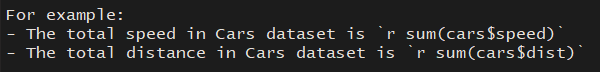
\includegraphics{C:/Users/gabriela.mourao/Documents/6-PESSOAL/R-files/TUTORIAL_MARKDOWN/Inline_code.png}
\caption{}
\end{figure}

\begin{center}\rule{0.5\linewidth}{\linethickness}\end{center}

\section{Formulas}\label{formulas}

\subsection{Inline and display mode}\label{inline-and-display-mode}

If you are typing just a small formula, you might just want to add it in
the line that you are typing. for example: ``This is an inline example
formula: \(E=mc^2\)''

\begin{verbatim}
      "This is an inline example formula: $E=mc^2$"
\end{verbatim}

But, if you are typing a very long expression, you might think that is
better to use the display mode:
\[a^n + b^n = (a - b)(a^{n-1} + a^{n-2}b + a^{n-3}b^2 + ... + ab^{n-2} + b^{n-1})\]

\begin{verbatim}
   $$a^n + b^n = (a - b)(a^{n-1} + a^{n-2}b + a^{n-3}b^2 + ... + ab^{n-2} + b^{n-1})$$
\end{verbatim}

\subsection{Symbols:}\label{symbols}

Some useful symbol formatations:

\begin{longtable}[]{@{}ccc@{}}
\toprule
Symbol & Latex & Comment\tabularnewline
\midrule
\endhead
\(\pm\) & \texttt{\textbackslash{}pm} & plus or minus\tabularnewline
\(\div\) & \texttt{\textbackslash{}div} & divided by\tabularnewline
\(\times\) & \texttt{\textbackslash{}times} & times\tabularnewline
\(\ge\) & \texttt{\textbackslash{}ge} & greater or equal\tabularnewline
\(\le\) & \texttt{\textbackslash{}le} & less or equal\tabularnewline
\(\forall\) & \texttt{\textbackslash{}forall} & For all\tabularnewline
\(\ne\) & \texttt{\textbackslash{}ne} & Not equal\tabularnewline
\(\sim\) & \texttt{\textbackslash{}sim} & is similar to\tabularnewline
\(\in\) & \texttt{\textbackslash{}in} & is member of\tabularnewline
\(\mathbb{R}\) & \texttt{\textbackslash{}mathbb\{R\}} & Set of real
numbers\tabularnewline
\(\hat{y}\) & \texttt{\textbackslash{}hat\{y\}} & y hat\tabularnewline
\(\bar{y}\) & \texttt{\textbackslash{}bar\{y\}} & y bar\tabularnewline
\bottomrule
\end{longtable}

\subsection{Greek Letters}\label{greek-letters}

\begin{longtable}[]{@{}ccc@{}}
\toprule
Symbol & Latex & Comment\tabularnewline
\midrule
\endhead
\(\alpha\) & \texttt{\textbackslash{}alpha} & alpha\tabularnewline
\(\beta\) & \texttt{\textbackslash{}beta} & beta\tabularnewline
\(\Delta~and~\delta\) &
\texttt{\textbackslash{}Delta\ and\ \textbackslash{}delta} &
Delta\tabularnewline
\(\epsilon~and~\varepsilon\) &
\texttt{\textbackslash{}epsilon\ and\ \textbackslash{}varepsilon} &
epsilon\tabularnewline
\(\Gamma~and~\gamma\) &
\texttt{\textbackslash{}Gamma\ and\ \textbackslash{}gamma} &
Gamma\tabularnewline
\(\pi\) & \texttt{\textbackslash{}pi} & pi\tabularnewline
\(\Sigma~\sigma~\varsigma\) &
\texttt{\textbackslash{}Sigma\ \textbackslash{}sigma\ \textbackslash{}varsigma}
& Sigma\tabularnewline
\bottomrule
\end{longtable}

\subsection{Index}\label{index}

\[
\begin{align}
x_i, x_{i} && \text{(Subscript)}\\
x^2 && \text{(Superscript)}\\
x^2_i,~x^2_{i,j} && \text{(Combined)}\  
\end{align}
\]

\begin{verbatim}
x_i, x_{i} (Subscript)
x^2 (Superscript)
x^2_i, x^2_{i,j} (Combined)  
\end{verbatim}

\subsection{Expressions}\label{expressions}

\subsubsection{Square roots}\label{square-roots}

To indicate a square root, use \texttt{\textbackslash{}sqrt}:
\(\sqrt{x}\)

\begin{verbatim}
$\sqrt{x}$
\end{verbatim}

\subsubsection{Fractions}\label{fractions}

The fractions are displayed using \texttt{\textbackslash{}frac}
symbol:\\
\(x=\frac{1}{1+e^{\beta_0+\beta_{1}\times y}}\)\\
or adding a parantesis:\\
\(x=\left(\frac{1}{1+e^{\beta_0+\beta_{1}\times y}}\right)\)

\begin{verbatim}
$x=\frac{1}{1+e^{\beta_0+\beta_{1}\times y}}$   

$x=\left(\frac{1}{1+e^{\beta_0+\beta_{1}\times y}}\right)$
\end{verbatim}

\subsubsection{Summation expression}\label{summation-expression}

To add a summation sign, you can use \texttt{\textbackslash{}sum} and
combine it with the index syntax introduced above:
\(\sum_{i=1}^n(y_i-\hat{y})^2\)

\begin{verbatim}
$\sum_{i=1}^n(y_i-\hat{y})^2$
\end{verbatim}

\subsubsection{Others}\label{others}

\[\int_0^{a} x^k~dx\]

\begin{verbatim}
$$\int_0^{a} x^k~dx$$
\end{verbatim}

\[ \frac{\partial u}{\partial t}
   = h^2 \left( \frac{\partial^2 u}{\partial x^2}
      + \frac{\partial^2 u}{\partial y^2}
      + \frac{\partial^2 u}{\partial z^2} \right) \]

\begin{verbatim}
$$ \frac{\partial u}{\partial t}
   = h^2 \left( \frac{\partial^2 u}{\partial x^2}
      + \frac{\partial^2 u}{\partial y^2}
      + \frac{\partial^2 u}{\partial z^2} \right) $$
\end{verbatim}

\[\lim_{x \to +\infty} \frac{3x^2 +7x^3}{x^2 +5x^4} = 3\]

\begin{verbatim}
$$\lim_{x \to +\infty} \frac{3x^2 +7x^3}{x^2 +5x^4} = 3$$
\end{verbatim}

\subsection{Matrices}\label{matrices}

\[\mathbf{X} = \left[\begin{array}
{rrr}
2 & 4 & 6 \\
8 & 10 & 12 \\
14 & 16 & 18
\end{array}\right]\]

\begin{verbatim}
$$\mathbf{X} = \left[\begin{array}
{rrr}
2 & 4 & 6 \\
8 & 10 & 12 \\
14 & 16 & 18
\end{array}\right]$$
\end{verbatim}

For operations with matrix you can also use
\(\mathbf{y}=\mathbf{X}\beta\), for example.

\begin{verbatim}
$\mathbf{y}=\mathbf{X}\beta$
\end{verbatim}

\subsection{Alignment and comments:}\label{alignment-and-comments}

You can use ``\textasciitilde{}'' to add some spaces in the formula:
\[ x_{i} + y_{i} \ge 0 ~~~~~~~\forall~i \in \mathbb{R} \]

\begin{verbatim}
$$ x_{i} + y_{i} \ge 0 ~~~~~~~\forall~i \in \mathbb{R} $$
\end{verbatim}

The formula inserted in ``index'' topic, wasn't completely shown at that
time. To write formulas together with comments, is necessary to use the
following syntax:

\begin{verbatim}
$$
\begin{align}
x_i, x_{i} && \text{(Subscript)}\\
x^2 && \text{(Superscript)}\\
x^2_i,~x^2_{i,j} && \text{(Combined)}\  
\end{align}
$$
\end{verbatim}

Besides that, when solving large expressions, might be useful to use
some alignment:

\[\begin{align}
      5\times a~+~10 &=30 \\
      5\times a &= 20 \\
      a &= 4
\end{align}\]

\begin{verbatim}
$$\begin
      5\times a~+~10 &=30 \\
      5\times a &= 20 \\
      a &= 4
\end$$
\end{verbatim}

\begin{center}\rule{0.5\linewidth}{\linethickness}\end{center}

\section{Links}\label{links}

To insert hyperlinks, you can type:
\href{https://www.rstudio.com}{R-studio} or
\url{https://www.rstudio.com}

\begin{verbatim}

[R-studio](https://www.rstudio.com)      
or     
https://www.rstudio.com   

\end{verbatim}

\begin{center}\rule{0.5\linewidth}{\linethickness}\end{center}

\section{Images}\label{images}

For images, the syntax is very similar to links:

\includegraphics{C:/Users/gabriela.mourao/Documents/6-PESSOAL/timon-studler-49992-unsplash.jpg}\footnote{photo
  by timon studler on unsplash}

\begin{verbatim}

![The amazing Hong Kong](C:/Users/gabriela.mourao/Documents/6-PESSOAL/timon-studler-49992-unsplash.jpg)^[photo by timon studler on unsplash]  

\end{verbatim}

\begin{center}\rule{0.5\linewidth}{\linethickness}\end{center}

\section{Tables}\label{tables}

Inserting manual tables in Rmarkdown is very easy:

\begin{longtable}[]{@{}cc@{}}
\toprule
Number Section & Section Name\tabularnewline
\midrule
\endhead
1.0 & Text Formatation\tabularnewline
2.0 & Output formats\tabularnewline
3.0 & Code options\tabularnewline
4.0 & Formulas\tabularnewline
5.0 & Links\tabularnewline
6.0 & Images\tabularnewline
7.0 & Tables\tabularnewline
\bottomrule
\end{longtable}

\begin{verbatim}
|Number Section|Section Name|
|:---:|:---:|
|1.0|Text Formatation|
|2.0|Output formats|
|3.0|Code options|
|4.0|Formulas|
|5.0|Links|
|6.0|Images|
|7.0|Tables|
\end{verbatim}

\section{References}\label{references}

Following are the references used in this tutorial. They are very
complete and useful, I sugest that you check it for more informations
about Rmarkdown.

\url{https://bookdown.org/yihui/rmarkdown/}
\url{https://oeis.org/wiki/List_of_LaTeX_mathematical_symbols}
\url{http://www.math.mcgill.ca/yyang/regression/RMarkdown/example.html}
\url{https://gist.github.com/derekmcloughlin/896da22518ef2f3d81b0}
\url{https://www.maths.tcd.ie/~dwilkins/LaTeXPrimer/Calculus.html}

\textbf{I hope you found this tutorial helpful! Cheers! :)}


\end{document}
